\documentclass[aspectratio=169]{beamer}
\usepackage[utf8]{inputenc}
\usepackage{amsmath,amssymb}
\usepackage{graphicx}
\usepackage{tikz}
\usetikzlibrary{shapes,arrows,positioning,calc}
\usepackage{hyperref}
\usepackage{xcolor}

% Custom 3B1B-inspired color palette
\definecolor{darkblue}{RGB}{10, 25, 47}
\definecolor{midblue}{RGB}{28, 73, 110}
\definecolor{lightcyan}{RGB}{116, 192, 227}
\definecolor{brownweight}{RGB}{140, 98, 57}
\definecolor{textgray}{RGB}{40, 40, 40}
\definecolor{bglight}{RGB}{248, 249, 250}

\setbeamercolor{palette primary}{bg=darkblue,fg=white}
\setbeamercolor{palette secondary}{bg=midblue,fg=white}
\setbeamercolor{palette tertiary}{bg=lightcyan,fg=darkblue}
\setbeamercolor{structure}{fg=midblue}
\setbeamercolor{background canvas}{bg=bglight}
\setbeamercolor{normal text}{fg=textgray}

\setbeamertemplate{navigation symbols}{}
\setbeamertemplate{footline}{
  \hfill\usebeamercolor[fg]{page number in head/foot}\usebeamerfont{page number in head/foot}
  \insertframenumber\,/\,\inserttotalframenumber\kern2em\vskip2pt
}

\title{Lecture 2: Inside the Transformer}
\subtitle{Word Embeddings, The Residual Stream, and Softmax Math}
\author{Transformer Lectures Series}
\date{Based on 3Blue1Brown Lessons}

\begin{document}

% Slide 1: Title Slide
\begin{frame}[plain]
  \titlepage
\end{frame}

% Slide 2: Word Embeddings and Vector Dimensions
\begin{frame}{Word Embeddings: Meaning as Vectors}
  \begin{itemize}
    \item Every token $i$ is converted into a vector $v_i \in \mathbb{R}^d$.
    \item **Dimensionality ($d$)**: 
      \begin{itemize}
        \item GPT-2 Small: $d = 768$
        \item GPT-3: $d = 12,288$
      \end{itemize}
    \item \textbf{Visualizing Coordinates}: If you have a 12,288-dimensional space, each coordinate represents some subtle, abstract linguistic concept (e.g., degree of politeness, association with water, gender, tense).
    \item These coordinates are learned parameters during training, not pre-programmed.
  \end{itemize}
\end{frame}

% Slide 3: Semantic Geometry & Vector Arithmetic
\begin{frame}{Geometric Properties of Embeddings}
  In high-dimensional space, directions have semantic meanings.
  
  \begin{columns}
    \begin{column}{0.5\textwidth}
      \begin{block}{Vector Arithmetic}
        Because dimensions hold semantic meaning, we can perform math on vectors:
        \[
        v_{\text{King}} - v_{\text{Man}} + v_{\text{Woman}} \approx v_{\text{Queen}}
        \]
        \[
        v_{\text{Italy}} - v_{\text{Rome}} + v_{\text{Paris}} \approx v_{\text{France}}
        \]
      \end{block}
    \end{column}
    
    \begin{column}{0.5\textwidth}
      \begin{block}{Cosine Similarity}
        We measure semantic relatedness using the dot product or cosine of the angle between vectors:
        \[
        \text{Similarity}(a, b) = \frac{a \cdot b}{\|a\| \|b\|}
        \]
        Similar words cluster closely together.
      \end{column}
  \end{columns}
\end{frame}

% Slide 4: Positional Encoding
\begin{frame}{Positional Encoding: Adding Word Order}
  A basic transformer processes tokens as an unordered bag of words. To incorporate structure:
  
  \begin{itemize}
    \item We define a positional vector $p_j$ for each index $j$ in the sequence.
    \item \textbf{Addition}: The positional vector is added directly to the initial token embedding:
      \[
      x_j = e_j + p_j
      \]
      where $e_j$ is the semantic word embedding and $p_j$ is the positional encoding.
    \item \textbf{Design}: These positional vectors are constructed using sinusoidal functions of different frequencies, allowing the model to easily deduce relative and absolute positions.
  \end{itemize}
\end{frame}

% Slide 5: The Residual Stream
\begin{frame}{The Residual Stream: The Central Highway}
  How does data flow through the network?
  
  \begin{itemize}
    \item \textbf{The Core Concept}: The residual stream is the set of vectors representing tokens flowing through the layers of the model.
    \item Instead of each block completely rewriting the vector, blocks write \textbf{incremental adjustments} ($\Delta v$):
      \[
      v_{\text{out}} = v_{\text{in}} + \Delta v
      \]
    \item This enables:
      \begin{itemize}
        \item Easy gradient flow during training (prevents vanishing gradients).
        \item The model to use intermediate layers to refine semantic features step-by-step.
      \end{itemize}
  \end{itemize}
\end{frame}

% Slide 6: How Blocks Read and Write
\begin{frame}{How Blocks Interact with the Residual Stream}
  \centering
  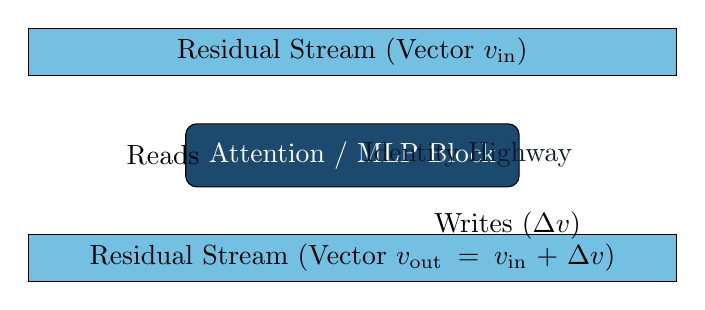
\begin{tikzpicture}[node distance=1.5cm, auto, >=latex]
    \tikzstyle{stream} = [draw, fill=lightcyan, text width=8cm, text centered, minimum height=0.6cm]
    \tikzstyle{block} = [draw, fill=midblue, text=white, text width=4cm, text centered, rounded corners, minimum height=0.8cm]
    
    \node [stream] (in) {Residual Stream (Vector $v_{\text{in}}$)};
    \node [block, below=0.6cm of in] (calc) {Attention / MLP Block};
    \node [stream, below=2cm of in] (out) {Residual Stream (Vector $v_{\text{out}} = v_{\text{in}} + \Delta v$)};
    
    \path[->, thick] (in.south) -- ++(-1.5,0) |- (calc.west) node[near end, left] {Reads};
    \path[->, thick] (calc.east) -| ++(1.5,-0.6) -- (out.north) node[near end, right] {Writes ($\Delta v$)};
    \path[->, ultra thick, darkblue] (in.south) -- (out.north) node[midway, right] {Identity Highway};
  \end{tikzpicture}
\end{frame}

% Slide 7: The Softmax Function
\begin{frame}{The Softmax Function: Scaling Predictions}
  At the output layer, the final token vector is projected to a vector of "logits" $x \in \mathbb{R}^V$ (where $V$ is vocabulary size). We apply \textbf{Softmax} to compute probabilities:
  
  \[
  P(i) = \text{Softmax}(x)_i = \frac{e^{x_i}}{\sum_{j=1}^V e^{x_j}}
  \]
  
  \begin{itemize}
    \item \textbf{Exponentiation}: Ensures all output values are strictly positive.
    \item \textbf{Normalization}: Divides by the sum so the entire vector sums to 1.
    \item \textbf{Amplification}: Naturally accentuates the maximum value while suppressing lower scores.
  \end{itemize}
\end{frame}

% Slide 8: Softmax Temperature
\begin{frame}{Controlling "Creativity": Softmax Temperature ($T$)}
  We can control the flatness of the output probability distribution by scaling logits by a temperature parameter $T$:
  
  \[
  P(i) = \frac{e^{x_i / T}}{\sum_{j=1}^V e^{x_j / T}}
  \]
  
  \begin{itemize}
    \item \textbf{Low Temperature ($T \to 0$)}:
      \begin{itemize}
        \item Accentuates differences; makes the model highly deterministic (greedy selection).
      \end{itemize}
    \item \textbf{High Temperature ($T > 1$)}:
      \begin{itemize}
        \item Flattens the distribution; increases randomness, diversity, and potential "creativity" or errors.
      \end{itemize}
  \end{itemize}
\end{frame}

% Slide 9: Stacking Architecture: A Complete Transformer Block
\begin{frame}{A Complete Transformer Block Stack}
  Mathematically, a single layer consists of:
  
  \begin{block}{Attention Layer Step}
    \[
    v' = v + \text{Attention}(v)
    \]
  \end{block}
  
  \begin{block}{Feed-Forward Layer Step}
    \[
    v'' = v' + \text{MLP}(v')
    \]
  \end{block}
  
  Both steps use **Layer Normalization** and skip connections (residual additions) to guarantee architectural stability.
\end{frame}

% Slide 10: Summary of Layer 2
\begin{frame}{Summary: Lecture 2 Recap}
  \begin{itemize}
    \item Words are projected into massive high-dimensional vector spaces (e.g., $d=12,288$).
    \item Semantics map to directions; word order is injected via positional encodings.
    \item The **Residual Stream** acts as the shared information highway. Blocks write adjustments ($\Delta v$), leaving the base path open.
    \item **Softmax** normalizes output logits, and **Temperature** scales output predictability.
  \end{itemize}
\end{frame}

\end{document}
